\section{Method}
\subsection{Time-stamped Transcript}
Several on-line video lecture platforms (e.g. Khan Academy) provide transcripts. In cases where transcripts were not provided, we used an on-line audio transcription service to acquire a verbatim text transcript. Then, we used a tool from \cite{rubin2013content} to compute an alignment between the video's audio file and the transcript. The final output is a time-stamped transcript, where each word is annotated with a start and end time.

\subsection{Stroke Extraction}
Visual content in blackboards-style lectures consists of \textit{strokes} drawn by the instructor on the board. Specifically, a \textit{stroke} is defined as the set of foreground pixels that is drawn during one continuous drawing activity. The method used to extract strokes from video frames is similar to that used by \cite{monserrat2013notevideo} to extract visual objects in their NoteVideo interface. By comparing the number of foreground pixels in consecutive frames, the start and end time of each drawing activity is detected. A noticeable increase in the foreground pixels signals start of drawing, while no change in the frames marks end of drawing. The difference between the end and start frames gives an image of the stroke drawn during that period. Figure~\ref{Fig:stroke_examples} shows examples of extracted strokes from different videos. A typical stroke comprises several characters to several words, or it can also be a part of a figure such as a graph (Figure~\ref{Fig:stroke_examples}c).  

\begin{figure}[h]
       \centering
        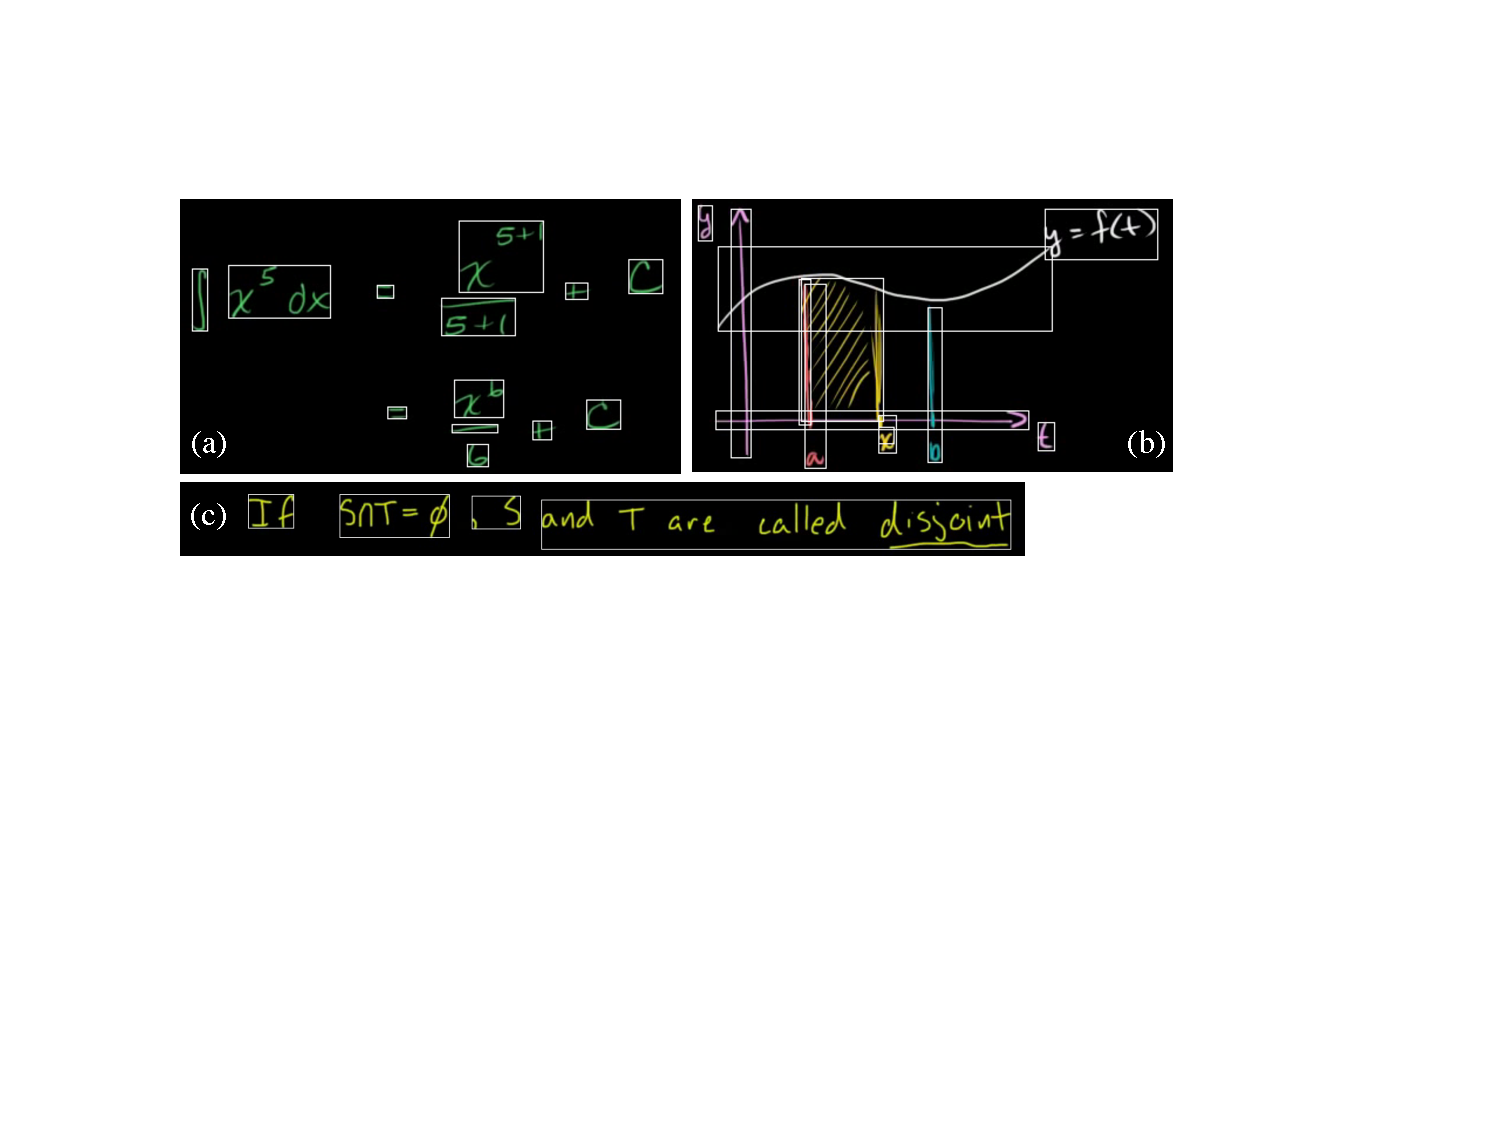
\includegraphics[width=0.45\textwidth, clip=true]{images/example_strokes}
        \caption{Examples of strokes extracted from different videos.}
        \label{Fig:stroke_examples}
\end{figure}

\subsection{Hierarchical Grouping of Strokes}
We group strokes into hierarchical units: lines and sentence-strokes.  
A line consists of a set of strokes that \textit{belong together} semantically. For example, a line could be a single row of equations, or a graph including its labels. Figure~\ref{Fig:line_examples} shows examples of lines. The problem of grouping strokes into lines is analogous to the problem of line breaking, also known as word wrapping \cite{knuth1981breaking}. An important difference is that in the traditional word wrapping problem, only a contiguous set of words can be put in the same line. In our case, strokes in a single line can be interspersed by strokes in a different line. This happens, for example, when the instructor goes back and forth between two lines of equations, or between a graph and an equation (Figures~\ref{Fig:line_order}). 

\subsubsection{Lines}
We use dynamic programming to group strokes into a set of lines. The algorithm iterates through the strokes, $s_i \in \mathbf{S}$, in the order of their appearance in the video, and keeps track of $L_i$, the optimal (determined by the scoring function described below) set of lines upto stroke $s_i$. For each new stroke, $s_\text{i+1}$, the algorithm considers all possible previous line breaks $L_j$, where $j < i+1$. For each $L_j$, it considers $\left\vert{L_j}\right\vert + 1$ possibilities: merging strokes $\{s_\text{j+1}, ... s_\text{i+1}\}$ with one of the lines $l_n \in L_j$, or adding a new line $\{s_\text{j+1}, ... s_\text{i+1}\}$ to $L_j$. The optimal solution among the $\sum_\text{j$<$i+1}{(\left\vert{L_j}\right\vert+1)}$ possibilities is $L_\text{i+1}$.   

The scoring function to determine the optimal set of lines is based on a number of observations: 

\textbf{Lines are compact.} Strokes that belong together are arranged in a compact figure. We consider three measures of compactness for a line: overall, horizontal and vertical. 
\begin{itemize}
\item Overall compactness of a line $l$is measured as 
\begin{equation}
c_1(l) = \frac{\sum\limits_{s\in l}area(\{s\})}{area(l)}
\end{equation}
where $area(\cdot)$ is the the bounding box area of a set of strokes. 
\item 
Intuitively, horizontal compactness is related to the maximum horizontal \textit{gap} between strokes within a line. Figure \ref{Fig:hv_compactness} shows an illustration of the of how gaps between strokes are measured. 
First, we define a horizontal projection function of a set of strokes, $S$, as 
\begin{equation}
proj_h(x, S}) = \big{|}\{s\in S \small{|} x_\text{min}(s)\le x \le x_\text{max}(s)\}\big{|}
\label{Eq:projh}
\end{equation}\\  
where $x_min(s)$, and $x_max(s)$ are the minimum and maximum $x$-coordinates of the bounding box of $s$ respectively. Then, the maximum horizontal gap of a line $l$ is
\begin{equation}
x_\text{gap}(l) = \argmax_{x_i, x_\text{i+1} \in proj_{h}(x,l)\ne 0}} (x_\text{i+1} - x_i)
\end{equation}
and horizontal compactness is defined as:
\begin{equation}
c_2(l) = -x_\text{gap}(l)
\end{equation}
\item Vertical compactness is defined similarly, in terms of a vertical projection function, $proj_{v}$, and the maximum vertical gap, $y_\text{gap}$.
\begin{equation}
proj_v(y, S}) = \big{|}\{s\in S \small{|} y_\text{min}(s)\le y \le y_\text{max}(s)\}\big{|}
\label{Eq:projv}
\end{equation}
\begin{equation}
y_\text{gap}(l) = \argmax_{y_i, y_\text{i+1} \in proj_{v}(y,l)\ne 0}} (y_\text{i+1}
- y_i)
\end{equation}
\begin{equation}
c_3(l) = -y_\text{gap}(l)
\end{equation}
\end{itemize}

\textbf{Strokes within a line are aligned horizontally.} With the exception of certain elements in graphs or figures, most lines comprising equations or words are written left to right. The strokes in such lines are aligned horizontally. We compute the maximum number of horizontally aligned strokes in each line, using the vertical projection function in Equation (\ref{Eq:projv}).
\begin{equation}
n_\text{align}(l) = \argmax_{y_\text{min}(l) \le y \le y_\text{max}(l)} proj_v(y)
\label{Eq:n_align}
\end{equation}

\textbf{Lines are spatio-temporally separate from each other.} This observation is complementary to the first observation, i.e. lines are compact. Whereas strokes that belong together are written close together. We express this property by penalizing overlap between distinct lines, measured by the overlapping area between their bounding boxes.
\begin{equation}
p_\text{overlap}(l_i, l_j) = \frac{area(l_i\cap l_j)}{min(area(l_i), area(l_j))}
\end{equation}
A similar property holds in the temporal domain. After writing a single line and before going to the next line, there is a brief pause while the instructor moves the cursor to the next position or adds some explanation. In order to enforce this property, we compute the temporal distance between two consecutive strokes across line-breaking points.
\begin{equation}
t_\text{dist}(s_i, s_\text{i+1}) = start(s_\text{i+1}) - end(s_i)
\end{equation}
where $s_i \in l_m$ and $s_\text{i+1} \in l_n$ belong to different lines $(m \neq n)$, and $start(\cdot)$ and $end(\cdot)$ are start and end times of when the stroke is drawn in the video.

The first four features (compactness and horizontal alignment) are properties of individual lines. Together, these define a scoring function for the \textit{goodness} of a single line.
\begin{equation}
s_1(l) = \alpha_1c_1(l) + \alpha_2c_2(l) + \alpha_3c_3(l) + \alpha_4n_\text{align}(l)
\end{equation}

The last two features are properties of relationship between multiple lines, and defines a \textit{goodness} score for a set of lines. 
\begin{equation}
s_2(L) = -\sum \limits_{l_i,l_j\in L, i\neq j}p_\text{overlap}(l_i, l_j) +\sum \limits_{s_i\in l_m, s_\text{i+1} \in l_\text{n}, m \neq n}t_\text{dist}(s_i, s_{i+1})
\end{equation}

The final scoring function is a weighted average of the two scores.
Figure \ref{Fig:line_examples} shows results obtained from our line breaking algorithm. The algorithm successfully segments meaningful groups of strokes from different layouts of figures and equations.


\begin{algorithm}[h]
\DontPrintSemicolon
\SetAlgoLined
\SetCommentSty{\tiny\ttfamily} 
  \SetKwInOut{Input}{Input}\SetKwInOut{Output}{Output}
  \Input{list of strokes ${S}$}
  \Output{list of optimal lines, ${L_{\left\vert{S}\right\vert}}$}
  $L_{-1} =$ \string{\string} \tcp{$L_i=$ optimal set of lines upto $i$-th stroke}\
    \For{each stroke $s_i \in \mathbf{S}$}{
    \textit{minscore} = $+\infty$\;
    \For{$j \leftarrow -1$ \textbf{to} $i-1$}{
      \For{$n \leftarrow 0$ \textbf{to} $\left\vert{L_j}\right\vert+1$}{
        \tcp{score to merge $\{s_{j+1}, ..., s_i\}$ to $n$-th line of $L_j$}\
        \tcp{If $n = \left\vert{L_j}\right\vert+1$, $\{s_{j+1}, ..., s_i\}$ is a new line}\
        \textit{score} $\leftarrow$ line\_score($L_{j}$, $n$)\;
        \If {score \textless minscore}{
          ${optj} = j$\;
          ${optn} = n$\;
        }
      }
   }
   $L_i=$ merge $s_i$ to $optn$-th line of $L_{optj}$\;
}
\label{Alg:line_break}
\end{algorithm}

\begin{figure*}[h]
        \centering
        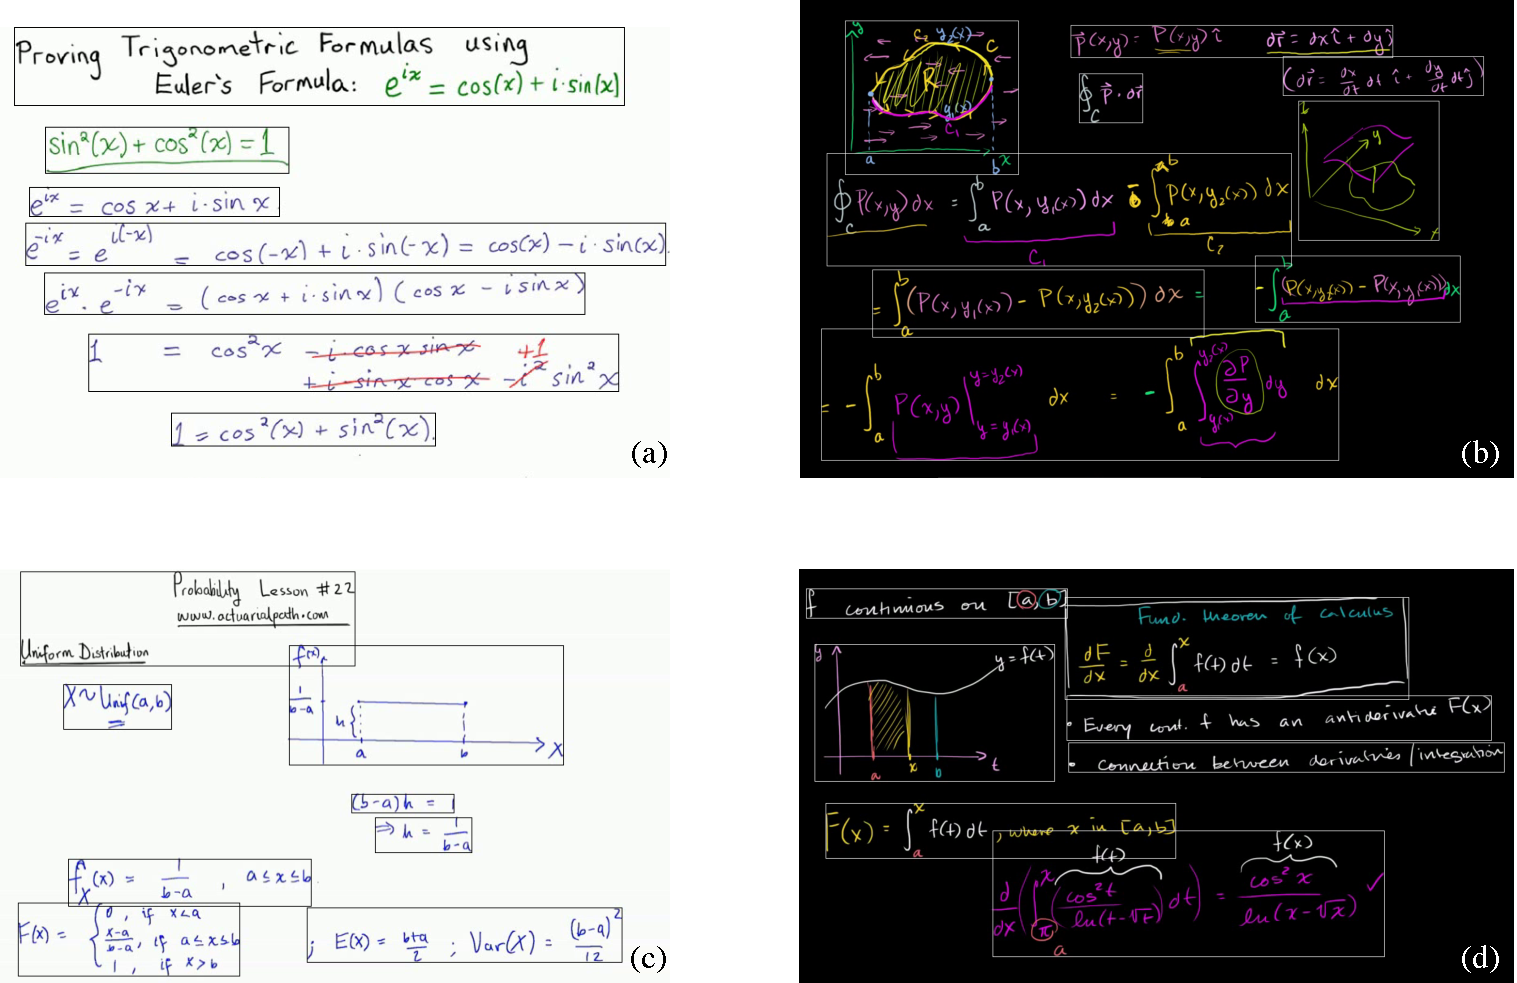
\includegraphics[width=0.9\textwidth]{images/example_lines}
        \caption{Examples of lines (i.e. set of strokes that belong together semantically) output from our line-breaking algorithm. Our algorithm successfully identifies meaningful groups even from complex layouts with a mix of equations, figures and graphs.}
        \label{Fig:line_examples}
\end{figure*}

\subsubsection{Sentence strokes}
If \textit{lines} represent meaningful segments in the video frames, sentences represent semantic units in transcripts. We further group strokes within each line into \textit{sentence strokes} using the temporal correspondence between strokes and transcript sentences. In summary, we have the following hierarchical grouping of strokes: strokes, sentence-strokes, and lines.



\subsection{Layout and Formatting}
We choose a static and linear format that aggregates the visual contents from the video and the transcript text in order to re-present the video content. A static format facilitates navigation of the content by presenting the entire video content in a single layout and  allowing the learners to go through it in their own pace. Moreover, lectures tend to be organized in a sequential structure that naturally lends itself to a linear layout. 

We observe two types sentences: sentences that describe the visual content without adding additional information (e.g.reading out the equation on the board), and sentences that provide further explanation (e.g. connection between different equations). The first type of sentence provide redundant information that is already present in the visual content. Figure~\ref{Fig:sentence_strokes} 


